\chapter{Implémentation} \label{implementation}
Ce chapitre décrit l'implémentation de l'application \textit{Virtual-Vertigo}. Des illustrations et des extraits de codes commentés ont été insérés afin de rendre les explications plus claires.

%%%%%%%%%%%%%%%%%%%%%%%%%%%%%%%%%%%%%%%%%%%%%%%%%%%%%%%%%%%%%%%%%%%%%%%%%%%%%%%%%%%%%%%%%%%%%%%%%%%%%%%%%%%%%%%%%%%%%%%%%%%

\section{Serveur Virtual-Vertigo}   \label{serveur2}
Le \textit{serveur NodeJS} mis en place utilise les \textit{modules ExpressJS et Socket.io}. Le \textit{module ExpressJS} a permis de créer le serveur Web, de rediriger les clients se connectant au serveur et de rendre les fichiers nécessaires publics. Le \textit{module Socket.io} a permis de créer un serveur utilisant les \textit{WebSockets} avec le serveur Web crée avec le module \textit{ExpressJS}. De plus, il permet de réceptionner les informations du \textit{Kinect} et de les renvoyer aux clients connectés. 

\lstset{style=mystyle} 
\begin{lstlisting}[language=JavaScript]
var express = require("express"), app = express(),
	server = require('http').createServer(app);

// redirection on /public who content the files 
app.use(express.static(__dirname + '/public'));

server.listen(3000, function(){// launch the server
  console.log('listening on *:3000');
});

//create the server socket using the server created with express
var io = require('socket.io').listen(server, { 'destroy buffer size': Infinity });
io.set('log level', 1);

//wait for the connections
io.sockets.on('connection', function(socket){
	console.info('Client connected');	
	// reception of datas captured by the kinect
	socket.on("squelette", function(json){
		io.sockets.emit("dataKinect", json);
	});
	socket.on("orientation", function(start, end, rotation){
		var json = {"start" : start, "end" : end, "rotation" : rotation };
		io.sockets.emit("boneOrientation", json);
	});
	socket.on('disconnect', function() {
		console.info('Client is gone');
	});
});
\end{lstlisting}

Ci-dessous un schéma illustrant l'échange de données entre le \textit{serveur Web Virtual-Vertigo}, les clients HTML et le Kinect.
\begin{figure}[H]
\centering
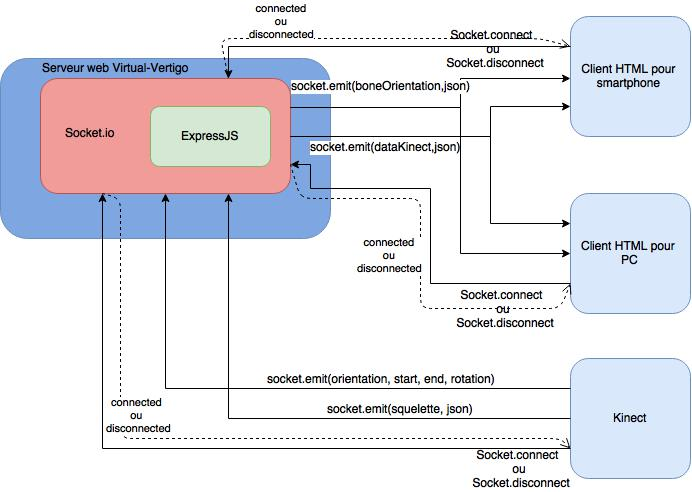
\includegraphics[scale=0.65]{serveur.jpg}
\caption{\label{schemaServeur} Illustration des échanges de données entre serveur, clients HTML et Kinect}
\end{figure}


%%%%%%%%%%%%%%%%%%%%%%%%%%%%%%%%%%%%%%%%%%%%%%%%%%%%%%%%%%%%%%%%%%%%%%%%%%%%%%%%%%%%%%%%%%%%%%%%%%%%%%%%%%%%%%%%%%%%%%%%%%%
\pagebreak
\section{Données provenant du Kinect}  \label{donnees}
Cette section décrit comment les données provenant du \textit{Kinect} ont été interprétées.

\subsection{Capture des données}  \label{capture}
La capture des données du \textit{Kinect} a été effectuée en C\# avec \textit{Visual Studio 2013}. Elle a été effectuée en plusieurs étapes : 
\lstset{language=[Sharp]C,
basicstyle=\footnotesize,
backgroundcolor=\color{backcolour}, 
captionpos=b,
frame=lines, % Oberhalb und unterhalb des Listings ist eine Linie
showspaces=false,
showtabs=false,
breaklines=true,
showstringspaces=false,
breakatwhitespace=true,
escapeinside={(*@}{@*)},
commentstyle=\color{greencomments},
morekeywords={partial, var, value, get, set},
keywordstyle=\color{bluekeywords},
stringstyle=\color{redstrings}
}

\begin{enumerate}
\item La connexion au \textit{serveur NodeJS} utilisant \textit{SocketIOC\# Client}.
\begin{lstlisting}
private static bool InitializeConnection(){
	var io = new SocketIOClient();
	socket = io.Connect("http://localhost:3000/");
	
	if (io.Connected)
		Console.WriteLine("kinect connected to server"); 
	else
		Console.WriteLine("failed to connect to server");
}
\end{lstlisting}

\item L'initialisation du \textit{Kinect}.
\begin{lstlisting}
private static void InitilizeKinect(){
	sensor = KinectSensor.KinectSensors.SingleOrDefault();
	if (sensor != null)
	{
		sensor.SkeletonStream.TrackingMode = SkeletonTrackingMode.Default;
		sensor.SkeletonStream.Enable(new TransformSmoothParameters()
		{
			Smoothing = 0.5f,
			Correction = 0.5f,
			Prediction = 0.5f,
			JitterRadius = 0.05f,
			MaxDeviationRadius = 0.04f
		});
		sensor.AllFramesReady += Sensor_AllFramesReady;

		sensor.Start();
		Console.WriteLine("sensor started");
	}
}
\end{lstlisting}

\item La capture et l'envoi de la position de chaque articulation captée du squelette.
\begin{lstlisting}
static void Sensor_AllFramesReady(object sender, AllFramesReadyEventArgs e) {
	using (var frame = e.OpenSkeletonFrame()) {
		if (frame != null){
			frame.CopySkeletonDataTo(skeletons);

			foreach (Skeleton skeleton in skeletons)
			{
				if (skeleton.TrackingState == SkeletonTrackingState.Tracked)
				{
					socket.Emit("squelette", skeleton.Joints);
					[...]
				}
			}
		}
	}
}
\end{lstlisting}

\item La récupération et l'envoi de l'orientation des mains afin de pouvoir voir la rotation de la main lors de la simulation.
\begin{lstlisting}
static void Sensor_AllFramesReady(object sender, AllFramesReadyEventArgs e) {
	[...]
	foreach (BoneOrientation orientation in skeleton.BoneOrientations)
	{
		if (orientation.StartJoint == JointType.WristLeft || orientation.StartJoint == JointType.WristRight)
				socket.Emit("orientation", orientation.StartJoint, orientation.EndJoint, orientation.AbsoluteRotation.Quaternion);
		}
	} 
}
\end{lstlisting}
\end{enumerate}

\subsection{Format des données}  \label{format}
Les données de positions envoyés au serveur sont au \textsf{format json} et sont des valeurs de la scène réelle. Les données sont envoyées dans un tableau où chaque élément est un \textsf{objet json} contenant les informations: 
\begin{itemize}
\item la valeur du point capté
\item le vecteur de position
\item l'état de l'articulation (captée, inférée ou non-captée), cette information n'est pas utilisée 
\end{itemize}

\begin{figure}[H]
\centering
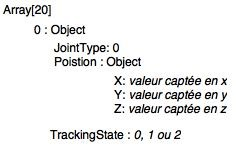
\includegraphics[scale=0.65]{jsonRecu.jpg}
\caption{\label{jsonrecu} Illustration de l'objet json des positions}
\end{figure}

Les données envoyées pour l'\textsf{orientation des mains} sont les suivantes : 
\begin{itemize}
\item le point d'origine, dans notre cas, le poignet
\item le point de fin, dans notre cas, la main
\item le vecteur d'orientation et l'angle de rotation en radians 
\end{itemize}

\begin{figure}[H]
\centering
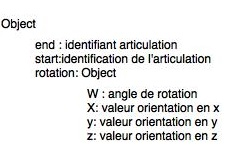
\includegraphics[scale=0.65]{jsonOrientation.jpg}
\caption{\label{jsonrecu} Illustration de l'objet json de l'orientation des mains}
\end{figure}
Pour plus d'informations sur les objets json, voir \cite{json}.

\subsection{Traitement des données} \label{traitement}
Selon le diagramme de séquence~\ref{sequence}, lorsque le serveur reçoit les données du Ki\textit{n}ect, il les renvoie aux clients HTML. Lorsque les clients HTML reçoivent à leur tour les données, celles-ci sont parcourues afin de faire correspondre les valeurs reçues avec une articulation du squelette (voir table des identificateurs d'articulations~\ref{valeurs}). Ces données sont réceptionnées dans un \textsf{nouvel objet json} contenant les informations: 

\begin{itemize}
\item le nom de l'articulation
\item la position x de l'articulation
\item la position y de l'articulation
\item la position z de l'articulation
\end{itemize}

\begin{figure}[H]
\centering
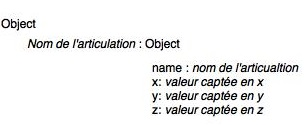
\includegraphics[scale=0.7]{jsonCreer.jpg}
\caption{\label{jsonrecu} Illustration de l'objet json créé avec les positions reçues et leurs articulations}
\end{figure}

A partir de cet \textsf{objet json}, le positionnement de chaque articulation peut être effectué. Au niveau des clients, un membre est représenté par deux sphères reliées par un cylindre. Afin d'adapter ces membres à la taille de chaque personne et d'animer ce personnage virtuel plusieurs étapes sont effectuées : 

\begin{itemize}
\item le calcul de la distance entre deux articulations reliées
\item le positionnement du membre entre les deux articulations
\item l'adaptation de la taille du membre en fonction de la distance calculée
\item le calcul de l'angle entre ses deux articulations en utilisant la fonction \texttt{atan2} (voir section~\ref{atan2})
\item la rotation du membre en fonction de l'angle calculé \\

\end{itemize} 
La description détaillée de chaque étape se trouve à la section~\ref{animation}. \\

Finalement, le déplacement du personnage selon l'avancement de la personne est effectué en se basant sur la position de sa tête. Tout ce traitement est effectué à la réception de chaque information du \textit{Kinect}. En effet, le \textit{Kinect} envoie un \textit{nouvel objet json} cycliquement.\\
Afin de rendre le personnage réaliste, l'ajout de membres réalistes par dessus les cylindres du personnage 3D serait envisageable. 

%%%%%%%%%%%%%%%%%%%%%%%%%%%%%%%%%%%%%%%%%%%%%%%%%%%%%%%%%%%%%%%%%%%%%%%%%%%%%%%%%%%%%%%%%%%%%%%%%%%%%%%%%%%%%%%%%%%%%%%%%%%
\pagebreak
\section{Modélisation de réalité virtuelle} \label{realiteVirtuelle}

\subsection{Création de la scène virtuelle}  \label{creation}
La création de la scène de réalité virtuelle a été réalisée avec \textit{X3DOM} (voir section~\ref{x3dom}). Afin d'ajouter de la 3D sur une simple page HTML, il faut impérativement avoir les fichiers suivants : 

\begin{itemize}
\item Le script x3dom.js permettant de manipuler la 3D
\item Le page de style x3dom.css afin d'utiliser la 3D \\

\end{itemize}

La création de la scène 3D est très simple, elle est basée sur un système de balises. Pour avoir la 3D sur la page, il y a plusieurs balises:

\begin{itemize}
\item la balise principale : \texttt{<x3d>}, 
\item la balise dans laquelle se trouve toute la scène 3D : \texttt{<scene>}, 
\item la balise permettant de définir de type de navigation(\texttt{examine}, \texttt{walk}, \texttt{fly}, etc.) : \texttt{<navigationinfo>},
\item la balise correspondant à la caméra : \texttt{<viewpoint>},
\item la balise permettant de dessiner des éléments 3D directement sur la page HTML : \texttt{<shape>}, 
\item les balises créer l'élément 3D voulu : \texttt{<box>, <sphere>, <cylinder>},
\item la balise permettant d'importer des scène 3D depuis Blender en format X3D : \texttt{<inline>}, 
\item la balise permettant de modifier l'élément 3D : \texttt{<transform>}.
\end{itemize}
Pour en savoir plus sur les balises voir \cite{NodesX3DOM}. \\
 

Chacune des balises utilisées doivent avoir un identifiant afin de pourvoir les manipuler. La manipulation de ces balises consiste à modifier ses attributs. L'accès aux balises s'effectue en \textit{JQuery}. Ci-dessous un exemple d'accès à une balise via son identifiant: 

\lstset{style=mystyle} 
\begin{lstlisting}[language=JavaScript]
$("#"+name).attr("translation");
\end{lstlisting}

Beaucoup de balises sont utilisées tel que \texttt{<navigationInfo>} afin de définir le mode \texttt{examin}. Cependant, seules deux balises utilisées sont modifiées au cours de la simulation. 
\begin{enumerate}
\item La balise \texttt{<transform>} est utilisée pour ses attributs suivants : 

\begin{itemize}
\item \texttt{translation} : déplace les balises se trouvant dans la balise \texttt{<transform>} dans la scène. Par exemple, le déplacement du personnage et de la caméra sur la planche.
\begin{lstlisting}[language=JavaScript]
$("#armature").attr("translation",  (parseFloat(position.head.z) - 4.0) + " 7.3 0");
$("#camera").attr("translation", (parseFloat(position.head.z) - 4.0) + " 8 " + (parseFloat(position.head.x) -0.2) );		
\end{lstlisting}

\item \texttt{rotation} : effectue une rotation sur les balises se trouvant dedans dans la scène virtuelle. Par exemple, la rotation des immeubles à 90 degrés. 
\begin{lstlisting}[language=Html]
<transform id='immeuble' translation='0 0 0' rotation='0 1 0 1.57' >
    <inline url="./blender/vue_semi_finale.x3d"></inline>
 </transform>
\end{lstlisting} 
\end{itemize}

\item La balise \texttt{<viewpoint>} est utilisée pour ses attributs suivants :

\begin{itemize}
\item \texttt{position} : place la caméra aux coordonnées correspondantes. Par exemple, le placement initiale de la vue.
\begin{lstlisting}[language=Html]
<Viewpoint id="vpp" DEF='viewpoint' position="0 0 5" orientation='1 0 0 -0.2' centerOfRotation="0 0 5"  fieldOfView="2.0" ></Viewpoint>	
\end{lstlisting} 

\item \texttt{centerOfRotation} : position correspondant à l'origine lors de la rotation de la vue. Par exemple, l'avancement du personnage sur la planche. 
\begin{lstlisting}[language=JavaScript]	
vp.attr("position", (parseFloat(position.head.x) -0.2) + " " + (parseFloat(position.head.y) -0.2)+ " " + (parseFloat(position.head.z) -0.2));
vp.attr("centerOfRotation", (parseFloat(position.head.x) -0.2) + " " + (parseFloat(position.head.y) -0.2)+ " " + (parseFloat(position.head.z) -0.2));
			
\end{lstlisting}

\item \texttt{orientation} : quaternion correspondant à l'orientation de la caméra dans la vue. Par exemple, le déplacement lors des mouvements de la tête. 
\begin{lstlisting}[language=JavaScript]	
MYAPP.viewpoint.setAttribute("orientation", orientation[0].x + " " + orientation[0].y + " " + orientation[0].z + " " + orientation[1]);
\end{lstlisting}
\end{itemize}

\end{enumerate}


\subsection{Création des immeubles}  \label{immeubles}
Les immeubles ont été crées avec un logiciel 3D \textit{Blender et Cinema4D}. Pour ce projet, deux scène de réalité virtuelle ont été réalisées : \\

\begin{enumerate}

\item Une version basique, implémentée sur \textit{Blender} contient 3 immeubles, une planche et le sol. Elle est illustrée sur la figure~\ref{ModeleBlender} : \\

\begin{figure}[H]
	\centering
		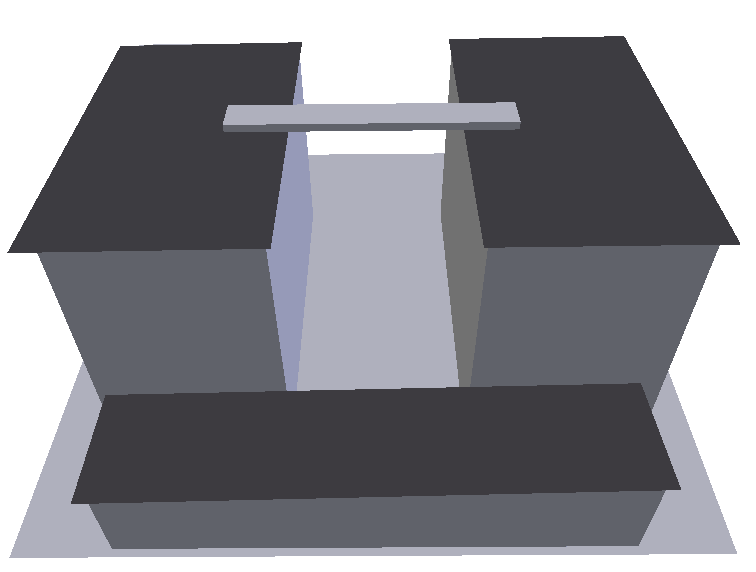
\includegraphics[scale=0.25]{ModeleBlender.png}
	\caption{\label{ModeleBlender} Modèle de vue 3D modélisé sur Blender}
\end{figure}

\item Afin de rendre la vue virtuelle plus réaliste, nous avons contacté \textsc{M. Olivier Donzé}, professeur de la filière architecture de paysage, et son assistant, \textsc{M. Benjamin Dupont-Roy} , qui travaillent sur la modélisation 3D du territoire. \\
La deuxième version,  réalisée par \textsc{M. Benjamin Dupond-Roy}, est plus détaillé et plus réaliste. Elle a été implémentée sur \textit{Cinema4D}. Il a modélisé la rue devant hepia en la personnalisant un peu. Voici quelques vues de son travail : \\

\begin{figure}[H]
   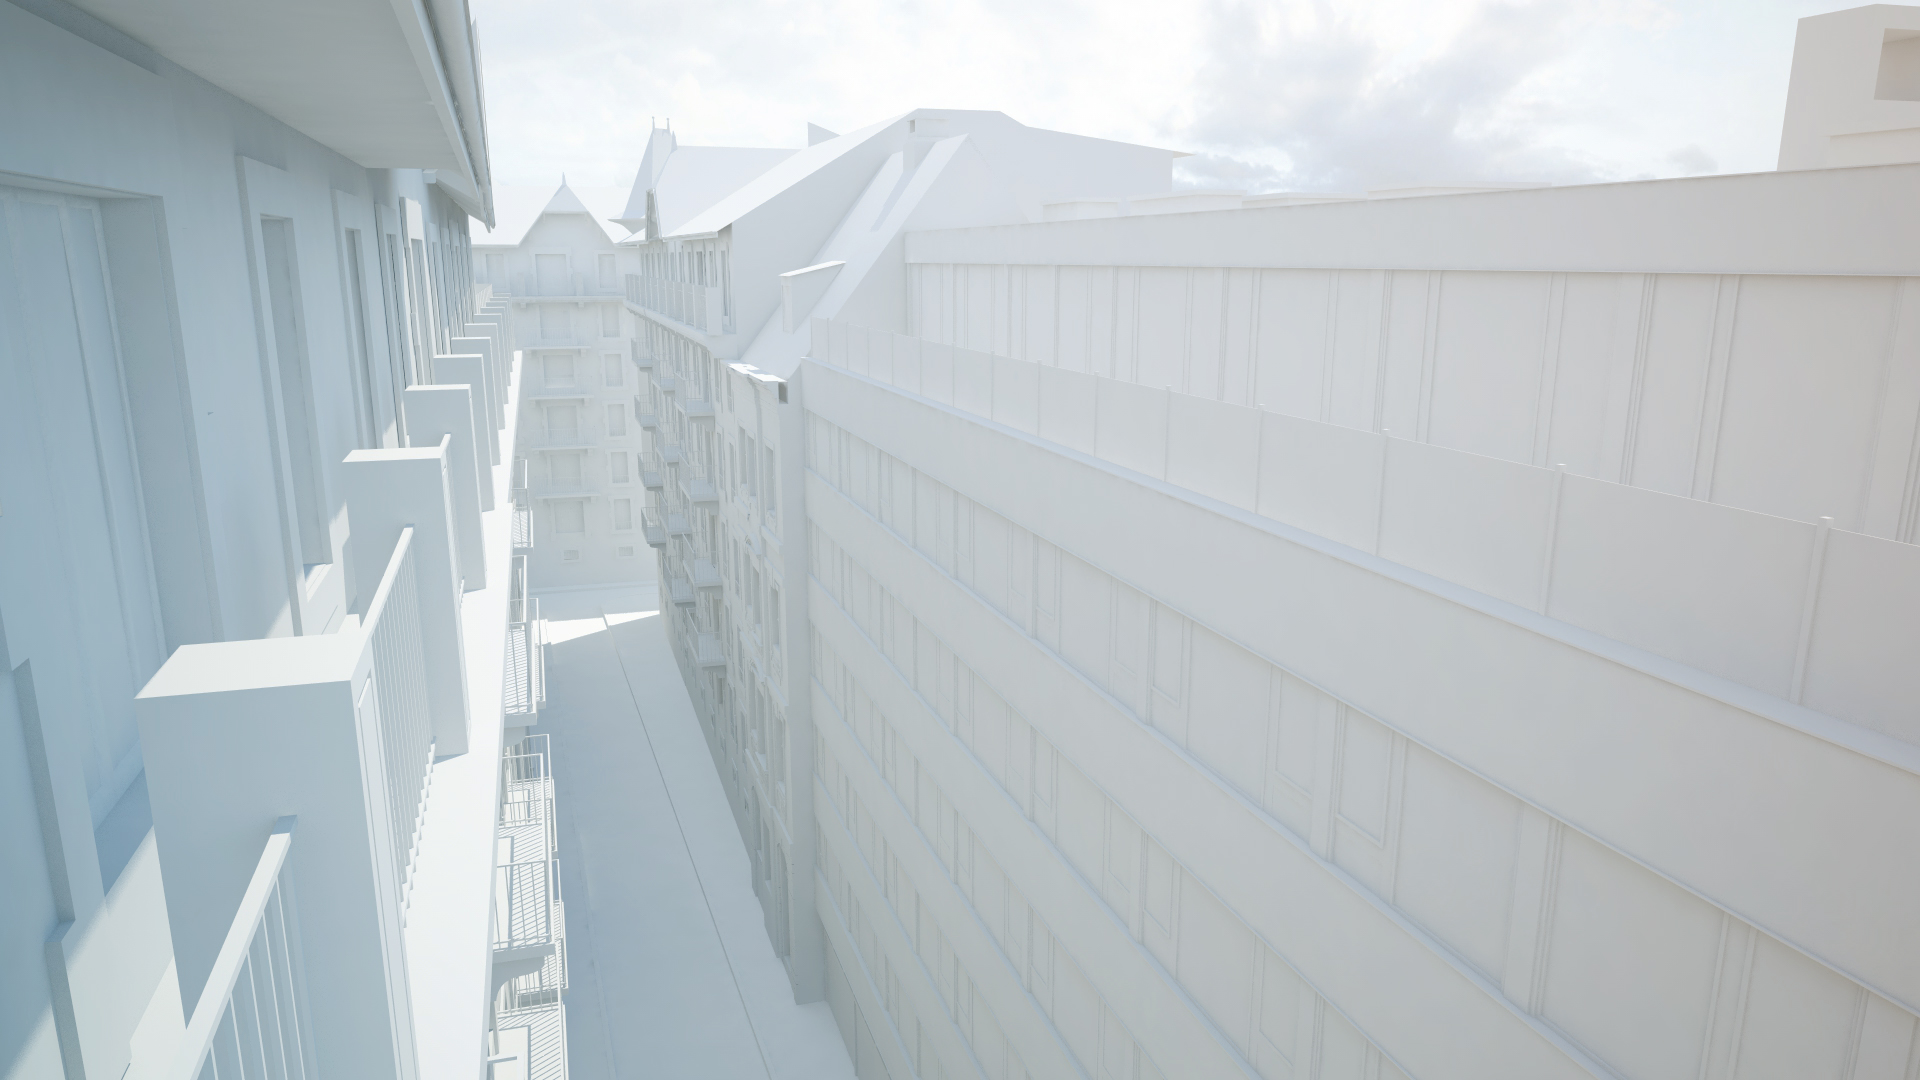
\includegraphics[scale=0.1]{Vue_balcon_OK.jpg}
   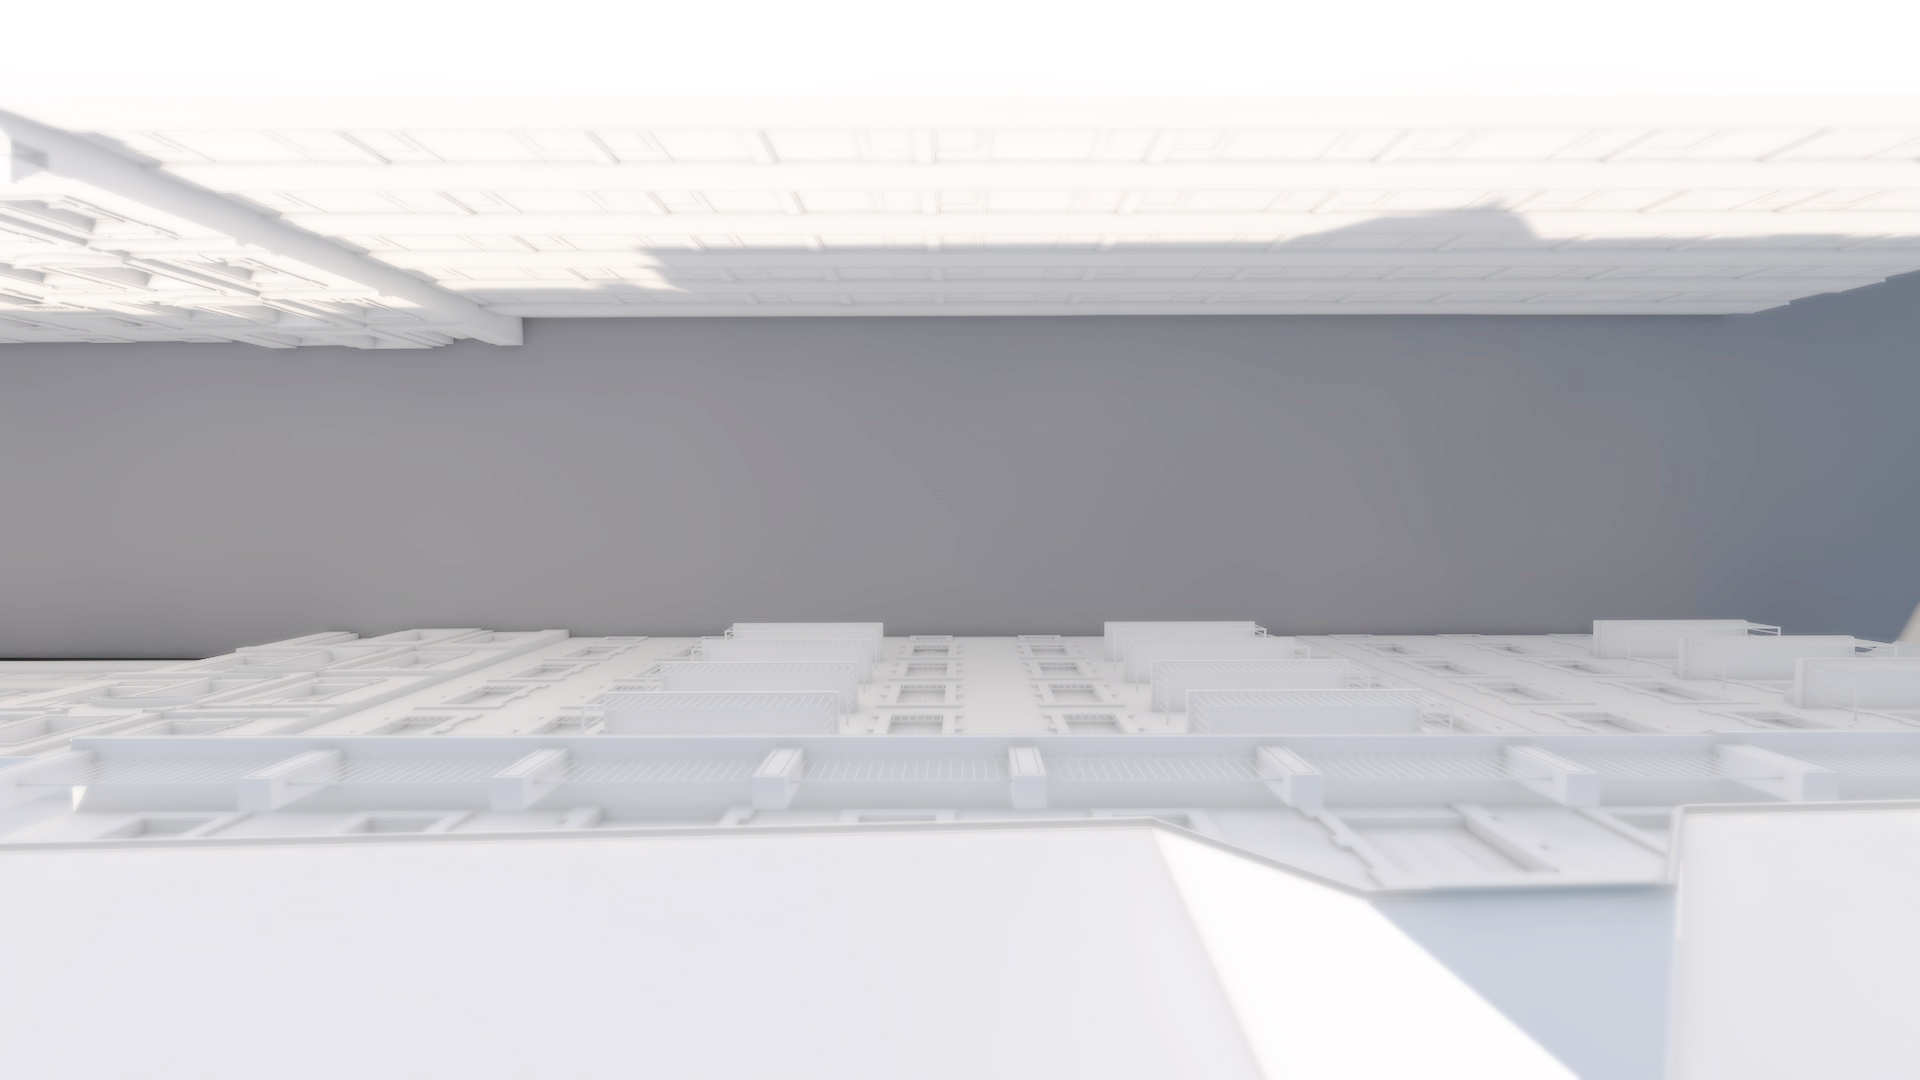
\includegraphics[scale=0.1]{Vue_2_ok.jpg}
   \caption{\label{vue 1 et 2} vue entre immeubles et du dessus}
\end{figure}
\begin{figure}[H]
   \includegraphics[scale=0.1]{Vue_rue_ok.jpg}
   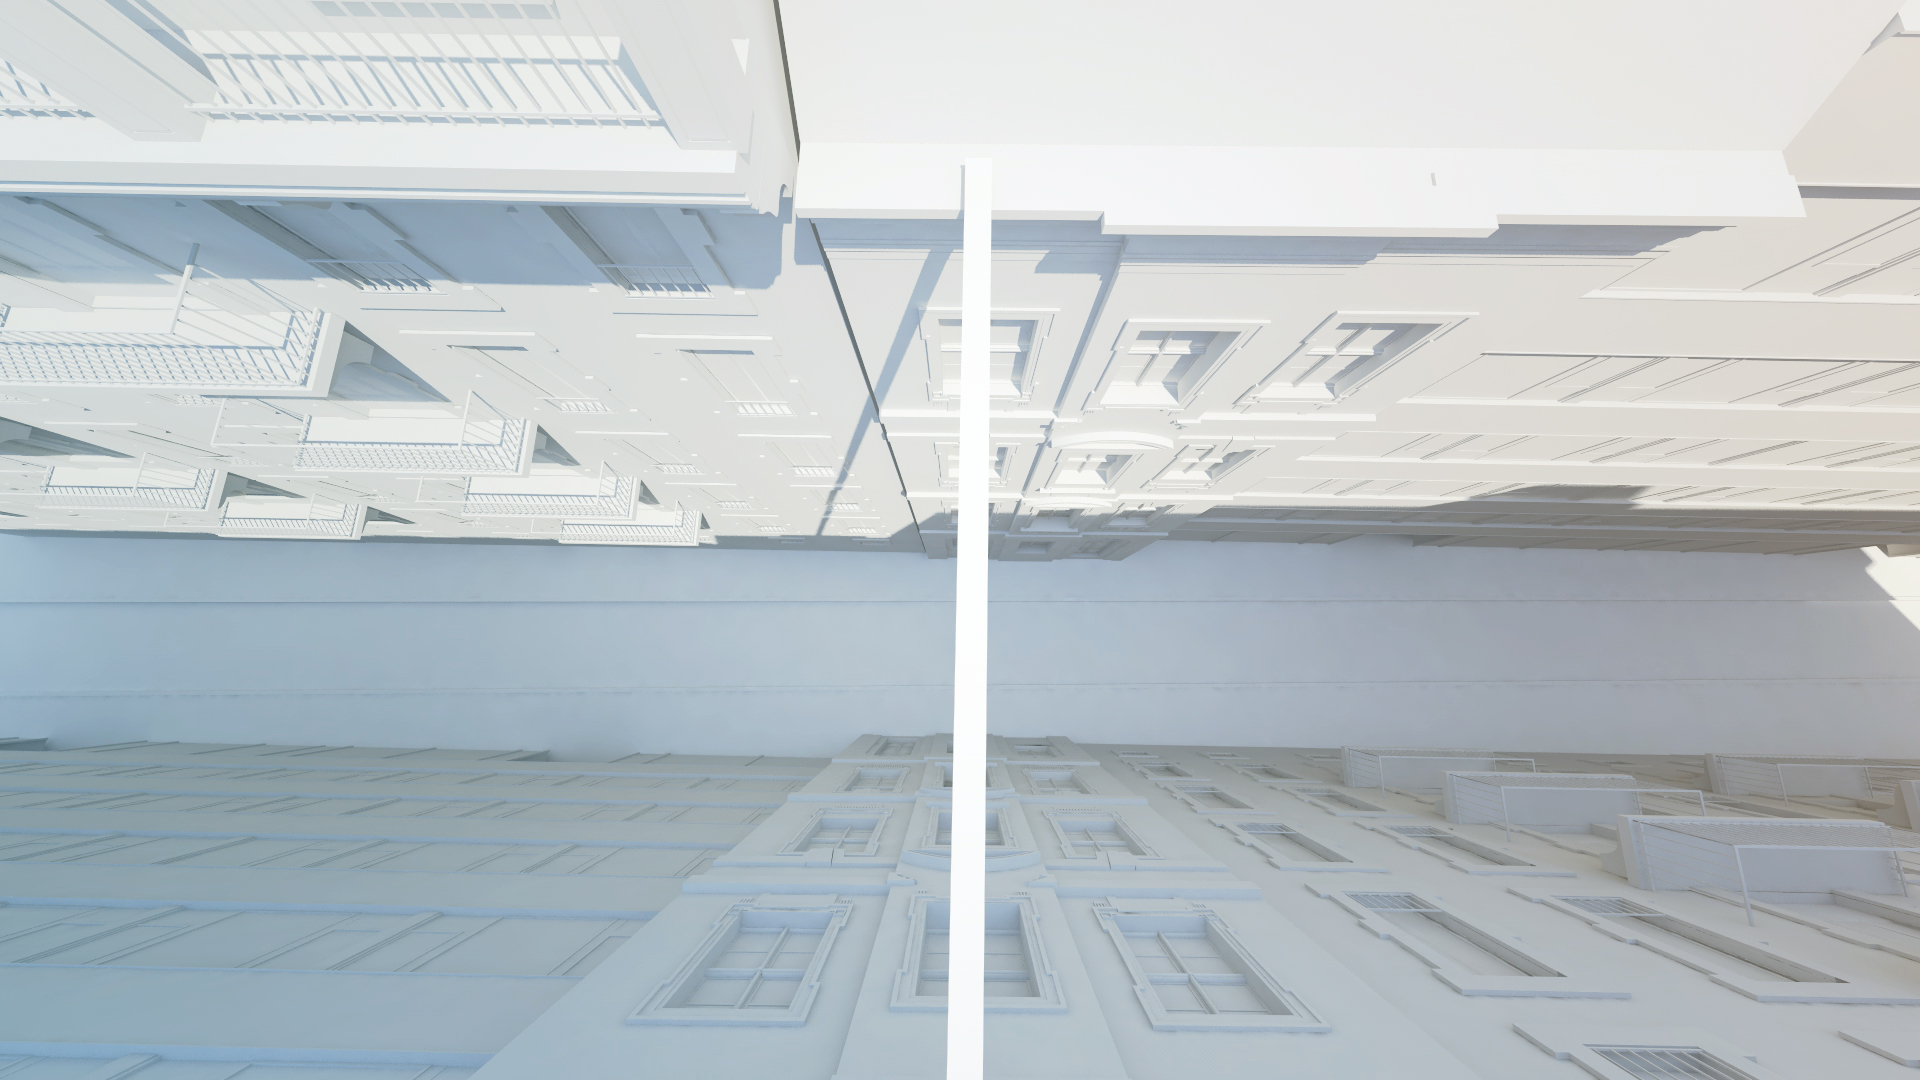
\includegraphics[scale=0.1]{Vue_planche_OK.jpg}
   \caption{\label{vue 3 et 4} vue depuis la rue et depuis la planche}
\end{figure}

\end{enumerate}

\subsection{Création du personnage}  \label{personnages}

La création du personnage a changé plusieurs fois lors de ce projet. Dans un premier temps, une femme avait été modélisée sur \textit{Blender} mais n'étant pas assez réaliste, celle-ci n'a plus été utilisée. \\
Puis, en utilisant \textit{MakeHuman} un homme réaliste a été créé et un squelette lui a été ajouté afin de l'animer si possible.
Cet homme a été utilisé pendant une grande partie du projet mais lorsqu'il a fallu l'animer il ne convenait plus. En effet, un problème d'export sous \textit{Blender} rendait le personnage rigide (pour plus de détails voir section~\ref{animationPersonnage}). \\
Finalement, afin de pouvoir animer un personnage en fonction du \textit{Kinect}, un squelette a été recréé en 3D. L'animation du personnage a été privilégiée par rapport à un rendu réaliste car priorité était de voir ses membres bouger lorsque l'on porte les \textit{Google CardBoard}. \\

Ci-dessous une illustration montrant l'"évolution" du personnage 3D tout au long du projet.
\begin{figure}[H]
	\centering
   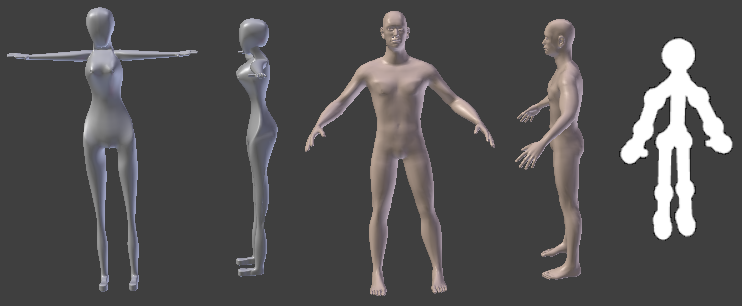
\includegraphics[scale=0.4]{Personnages.png}
   \caption{\label{Evopersonnages} "Evolution" du personnage 3D}
\end{figure}


\subsection{Textures}  \label{textures}
La pose des textures, dans le cas des deux modélisations, a été effectuée à partir des logiciels 3D \textit{Blender et Cinema4D}. En effet, lorsque la vue 3D est exportée en \textit{X3D}, les textures appliquées restent sur la vue. Il faut cependant avoir à disposition les textures lors du chargement sur \textit{X3DOM}. \\

Pour la vue basique à gauche, les textures ont été trouvées sur internet puis appliquées sur \textit{Blender} et pour la vue plus réaliste à droite, une photo a été prise et extrapolée pour bien se fondre sur les immeubles.\\

Ci-dessous une illustration du rendu 3D avec textures au bord de la planche.
\begin{figure}[H]
   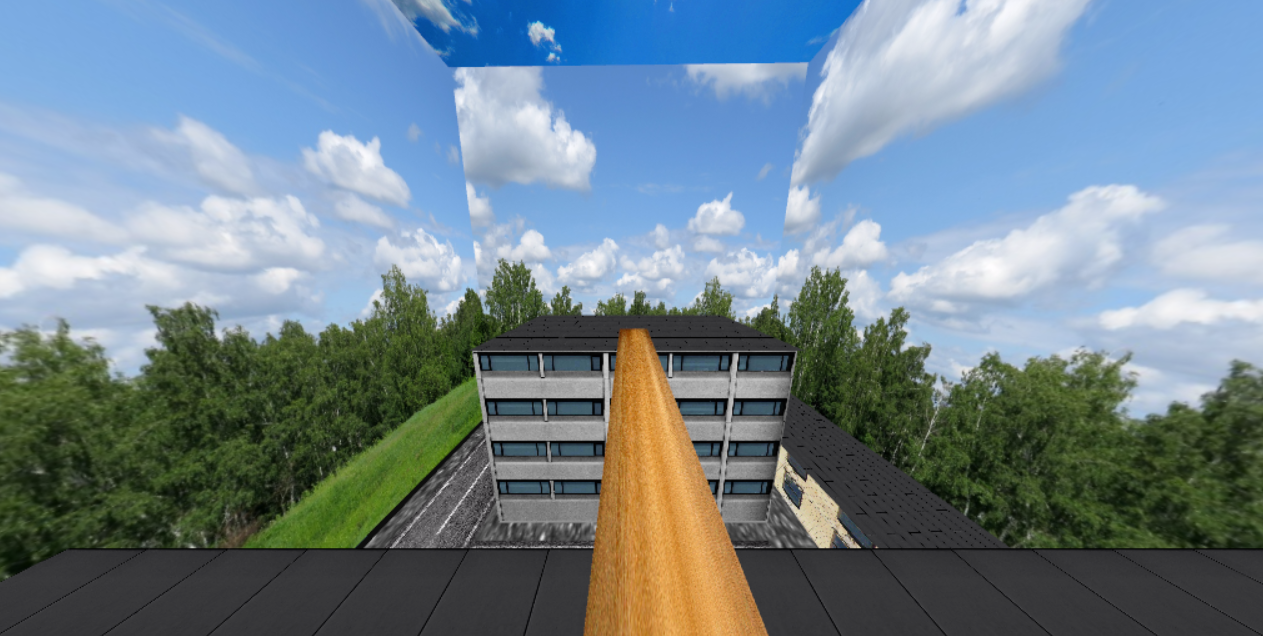
\includegraphics[scale=0.202]{vueBasiqueTextures.png}
   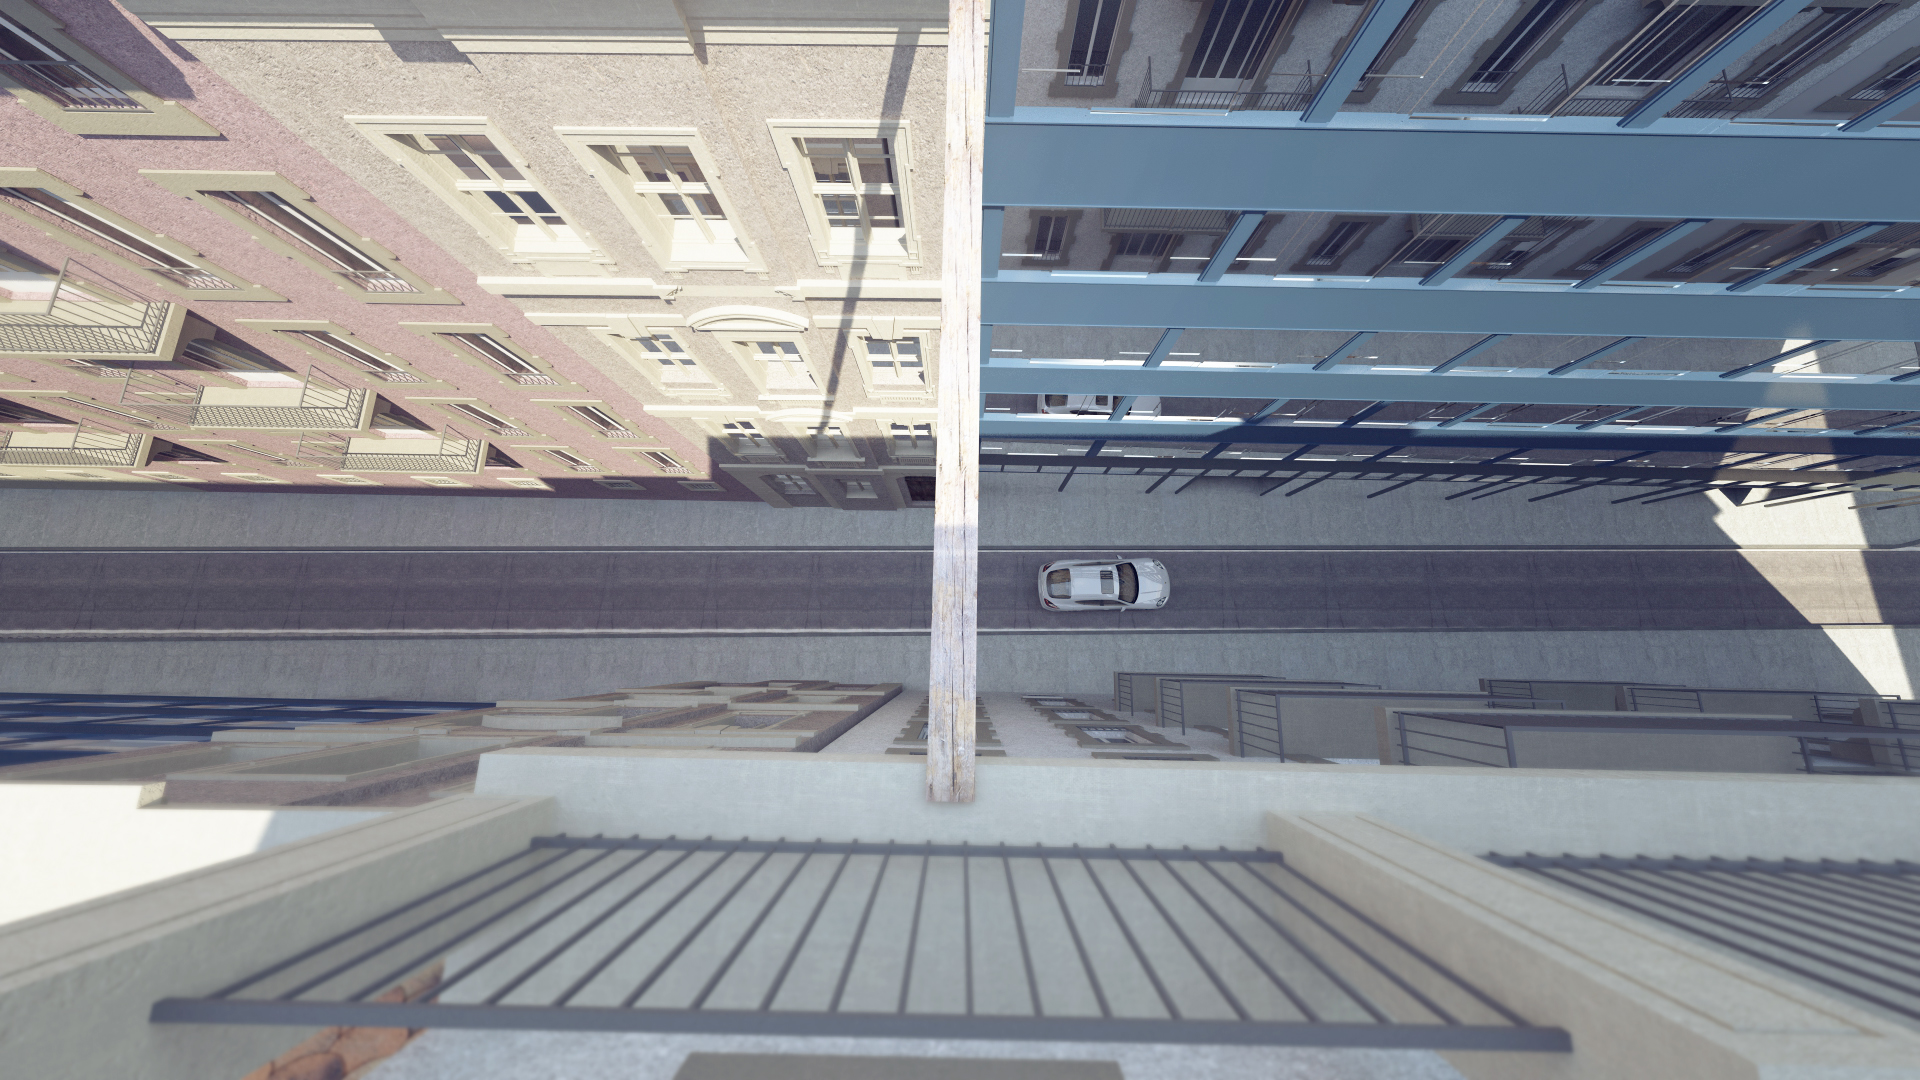
\includegraphics[scale=0.09]{Vue_planche2_ok.jpg}
   \caption{\label{textures} Illustrations vue virtuelle avec textures}
\end{figure}

%%%%%%%%%%%%%%%%%%%%%%%%%%%%%%%%%%%%%%%%%%%%%%%%%%%%%%%%%%%%%%%%%%%%%%%%%%%%%%%%%%%%%%%%%%%%%%%%%%%%%%%%%%%%%%%%%%%%%%%%%%%%
\pagebreak
\section{Animations sur la réalité virtuelle} \label{animation}
La prise en charge des différentes animations de la réalité virtuelle est locale au périphérique exécutant l'application.

\subsection*{Placement de la caméra}  \label{camera}
Le placement de la caméra s'effectue avec la balise \texttt{<viewpoint>}, en utilisant son attribut \texttt{position} correspondant au vecteur de position. Avec cette balise, il est possible de placer la caméra à la position de la tête.\\
Sur la vue du \textsf{smartphone}, la caméra se place en même temps que la tête avance. Il faut pour cela mettre à jour cet attribut à chaque changement.\\
Sur la vue de l'ordinateur, la caméra peut se déplacer comme sur la vue du \textsf{smartphone} ou être à un point fixe derrière la personne. Ces deux points de vues donnent une perspective différente.\\

A noter que la balise \texttt{<viewpoint>} est englobée par une balise \texttt{<transform>} qui permet d'effectuer une rotation suivi d'une translation. La rotation permet à la caméra de se placer perpendiculairement aux immeubles. La translation déplace la caméra sur un seul axe sans avoir à changer la position initiale de la caméra. \\ 

L'illustration~\ref{positionsCamera} ci-dessous montre la position de la caméra sur le \textsf{smartphone} et les deux positions de caméra possibles sur l'écran standard.
\begin{figure}[H]
\centering
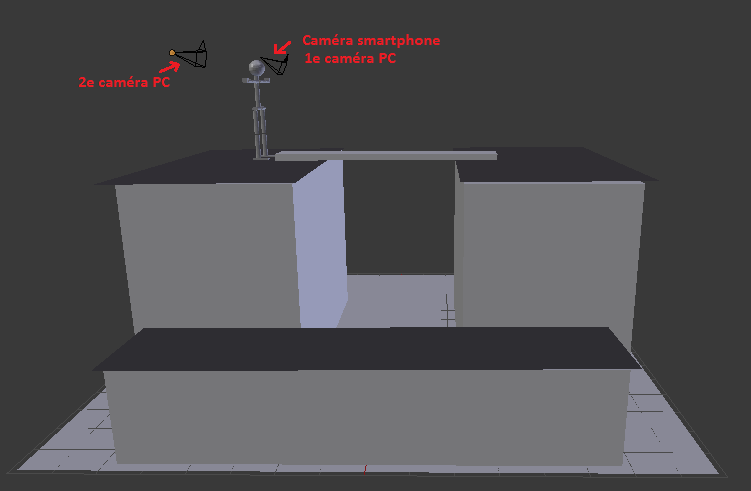
\includegraphics[scale=0.5]{positionCamera.png}
\caption{\label{positionsCamera} Illustrations des positions possibles de la caméra}
\end{figure}

\pagebreak
\subsection*{Orientation de la tête}  \label{orientation}
L'orientation de la tête s'effectue en utilisant l'accéléromètre du \textsf{smartphone}. L'accéléromètre mesure la force d'accélération appliquée au \textsf{smartphone} sur les axes x, y et z (force de gravitation). Il est utilisé pour détecter les mouvements. L'illustration~\ref{accelerometre} ci-dessous illustre les axes de l'accéléromètre.
\begin{figure}[H]
\centering
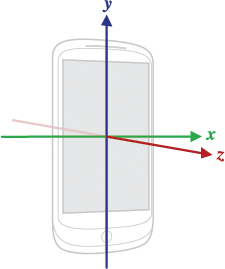
\includegraphics[angle=90,origin=c,scale=0.4]{accelerometre.png}
\caption{\label{accelerometre} Illustration des axes de l'accéléromètre}
\end{figure} 

La rotation de la vue en fonction des mouvements de la tête s'effectue en plusieurs étapes :

\begin{enumerate}
\item récupérer la rotation du \textsf{smartphone} dans un quaternion en utilisant des paramètres mis à disposition par \textit{X3DOM}
\begin{lstlisting}
var q0 = x3dom.fields.Quaternion.axisAngle(new x3dom.fields.SFVec3f(0,0,1),-deg2rad(window.orientation));		       
\end{lstlisting}

\item créer un quaternion avec les valeurs de l'accéléromètre
\begin{lstlisting}
var q = new x3dom.fields.Quaternion();
q.setFromEulerYXZ(deg2rad(MYAPP.deviceOrientation.beta), deg2rad(MYAPP.deviceOrientation.alpha), -deg2rad(MYAPP.deviceOrientation.gamma));
\end{lstlisting}

\item créer un quaternion afin de tourner la caméra car l'orientation captée par le \textsf{smartphone} pointe vers le haut
\begin{lstlisting}
var q1 = new x3dom.fields.Quaternion.axisAngle(new x3dom.fields.SFVec3f(1,0,0),-Math.PI/2); 
\end{lstlisting}

\item multiplier le quaternion des valeurs de l'accéléromètre avec les deux autres quaternions
\begin{lstlisting}
q = q.multiply(q1);
q = q.multiply(q0);
\end{lstlisting}

\item transformer le quaternion des valeurs de l'accéléromètre en un vecteur de position avec un angle de rotation
\begin{lstlisting}
var orientation = q.toAxisAngle();
\end{lstlisting}

\item appliquer les valeurs de accéléromètre à l'attribut \texttt{orientation} de la caméra 
\begin{lstlisting}
MYAPP.viewpoint.setAttribute("orientation", orientation[0].x + " " + orientation[0].y + " " + orientation[0].z + " " + orientation[1]);
\end{lstlisting}
\end{enumerate}

\subsection*{Avancement sur la planche}  \label{avancement}
L'avancement du personnage sur la planche virtuelle s'est effectué en deux temps en modifiant les balises \textit{X3DOM} :\\


\begin{enumerate}
\item \textbf{Simulation du déplacement du personnage sur la planche : } \\
Pour mettre en place ce déplacement fictif, une récursivité a été implémentée. Toutes les secondes, la distance définie diminue. Le personnage est alors déplacé et la vue suit ce déplacement. Cette récursion tourne en boucle parce que lorsque la distance est égale à la distance minimum définie, les valeurs sont réinitialisées.

\begin{lstlisting}[language=JavaScript]	
function moveFictif(){
	timer--;
	character.attr("translation", timer +' 20 2');
	vp.attr("position",'0 10 '+ timer);
	vp.attr("centerOfRotation", '0 10 '+ timer);

	if (timer <= -MAX_Z)
		timer = MAX_Z;
	
	sleep(1);
	moveFictif();
}
\end{lstlisting}


\item \textbf{Avancement du personnage en fonction du \textit{Kinect} et selon la positon de la tête :} \\
Au commencement de la simulation, la personne se place face au \textit{Kinect} à environ 4 mètres de distance. Puis elle commence à avancer sur la planche en portant les lunettes. La vue affichée sur le \textsf{smartphone} sera adaptée en fonction de ces déplacements. Les membres peuvent être vus lors de la simulation. Pendant le déplacement, une vérification est effectuée afin de savoir si la personne a "chuté".

\begin{lstlisting}[language=JavaScript]	
function move(){
	if (position.head != undefined)
		if ((position.head.z > 3.90 & !start) ){
			start = true; 
			document.getElementById('music').play();
		}else if (position.head.z < 0.70 & start)
			start = false;

		if (start){
			// only the all armature move, the animation of the member is not handle here
			vp.attr("position", (parseFloat(position.head.x) -0.2) + " " + (parseFloat(position.head.y) -0.2)+ " " + (parseFloat(position.head.z) -0.2));
			vp.attr("centerOfRotation", (parseFloat(position.head.x) -0.2) + " " + (parseFloat(position.head.y) -0.2)+ " " + (parseFloat(position.head.z) -0.2));
			$("#armature").attr("translation",  (parseFloat(position.head.z) - 4.0) + " 7.3 0");
			$("#camera").attr("translation", (parseFloat(position.head.z) - 4.0) + " 8 " + (parseFloat(position.head.x) -0.2) );
			checkBoundries();

		}
	}
\end{lstlisting}
\end{enumerate}

\subsection*{Animation du personnage} \label{animationPersonnage}
L'animation du personnage était un aspect important du projet car on voulait que la personne puisse voir ses membres lors de la simulation. Au cours du développement, l'animation du personnage a posé quelques problèmes (voir le chapitre~\ref{problemes}). Comme mentionné dans la section~\ref{traitement}), l'animation du personnage a été effectuée en suivant les étapes : \\

\begin{enumerate}

\item \textbf{Distance en deux dimensions entre des points $A=(A_x,A_y)$ et $B=(B_x,B_y)$ :}
\begin{equation}
AB = \sqrt{(B_x - A_x)^2 + (B_y - A_y)^2}
\end{equation}

\item \textbf{Angle entre 2 points A et B : }
L'angle est calculé selon le triangle rectangle suivant : 

\begin{figure}[H]
\centering
	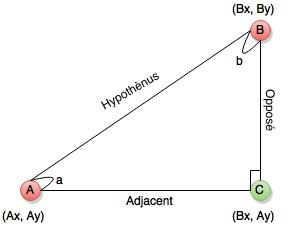
\includegraphics[scale=0.7]{Triangle.jpg}
	\caption{\label{triangle} Triangle rectangle utilisé pour le calcul de l'angle $a$}
\end{figure}

\begin{equation}
a = \mathrm{atan2}((B_y - A_y), (A_x - B_x))
\end{equation}
(La description de atan2 se trouve à la section~\ref{atan2}).\\

\item  \textbf{Positionnement du membre entre les points A et B :} une simple translation du cylindre correspondant à l'id à la position de l'articulation A. Le cylindre est positionné en fonction du point d'origine A et du point de fin B.

\begin{lstlisting}
function positionning(id, pos){
	$("#"+id).attr("translation", (pos.x) + " " +  (pos.y -0.5) + " " + pos.z);
}
\end{lstlisting}
\pagebreak
\item  \textbf{Adaptation de la taille du membre : } un \textsf{scaling} appliqué en x, correspondant à la longueur, au bon cylindre utilisant la distance calculée auparavant entre les 2 points~A~et~B.
\begin{lstlisting}
function scaling(id, distance, old){
	var distance = distance.toFixed(2);
	if (distance != old){
		$("#"+id).attr("scale", distance  +" "+ DIV_DISTANCE + " " + DIV_DISTANCE );
		old = distance;
	}
	return old;
}
\end{lstlisting}

\item \textbf{Rotation du membre : } une rotation est appliquée en z en utilisant l'angle calculé auparavant.
\begin{lstlisting}
function anime(id, angle, old){
	var angle = angle.toFixed(2);
	if (angle != old){
		$("#"+id).attr("rotation", "0 0 1 " + angle);
		old = angle;
	}
}
\end{lstlisting}
\end{enumerate}

A noter qu'un \textsf{objet json} a été mis en place contenant pour chaque membre relié : 
\begin{itemize}
\item un id correspondant à l'identification du cylindre 3D 
\item un membre A correspondant au membre de départ
\item un membre B correspondant au membre d'arrivé 
\end{itemize}

\begin{figure}[H]
\centering
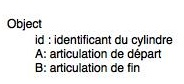
\includegraphics[scale=0.7]{jsonRelie.jpg}
\caption{\label{jsonrecu} Illustration de l'objet json des articulations reliées}
\end{figure}

A noter également que l'ordre des membres A et B est important pour l'animation. Car s'ils sont inversés l'animation se fera dans l'autre sens. Par exemple, si le membre A est le coude gauche et le membre B l'épaule gauche, le cylindre correspondant au bras sera placé aux positions du coude. Cela affecterait également la rotation du membre car le point de départ serait le coude.

\subsection*{Atan2} \label{atan2}
Atan2 est une variante de la fonction arc tangente prenant en paramètres deux valeurs. Pour tout paramètre réel non nul, atan2 est l'angle en radians entre la partie positive de l'axe des x d'un plan et le point de ce plan aux coordonnées passées en paramètres. L'angle donné est positif pour les angles dans le sens trigonométrique (sens anti-horaire) et négatif dans l'autre sens (pour plus d'information sur atan2 \cite{atan2}).
\pagebreak
\subsubsection{Définition et illustrations}
Pour $y \ne  \ 0$: \\
\begin{figure}[H]
	\centering
	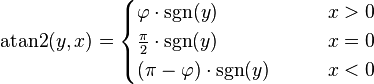
\includegraphics[scale=0.6]{atan2Y0.png} 
\end{figure}
où $\varphi $ \ est l'angle compris entre [0, $\Pi$ /2] de façon à ce que $\mathrm{tan}(\varphi) = |y/x|$ et sgn est la fonction signe. \\

Et: 
\begin{figure}[H]
	\centering
	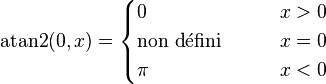
\includegraphics[scale=0.75]{atan22.png} 
\end{figure}

\begin{figure}[H]
	\centering
	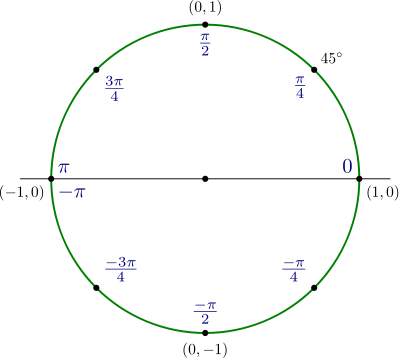
\includegraphics[scale=0.5]{atan2Circle.png} 
	\caption{\label{atan2circle} Illustration du cercle trigonométrique des valeurs de atan2}
\end{figure}
Le cercle ci-dessus illustre les valeurs, en radians, de atan2. Les angles sont inscris en bleu et les points sont inscris à l'extérieur du cercle. 


\subsection*{Effet sonore}  \label{sonore}
L'ajout d'un effet sonore lors de la simulation semblait indispensable afin de permettre à l'utilisateur mieux s'intégrer dans sa simulation. Cet effet sonore est un enregistrement du bruit ambiant à la fenêtre. Il a été ajouté en HTML5 et est activé, en \textsf{JavaScript}, lorsque la personne se trouve au bord de la planche.

\subsection*{Chute et recommencement}  \label{chute}
Une animation de "chute" a été implémentée. Lorsque la personne "chute", c'est-à-dire qu'elle a les deux pieds en dehors de la planche. La personne voit la vue descendre au fur et à mesure de la "chute". La désactivation cette option est possible si la personne ne le supporte pas. \\

La possibilité de recommencer la simulation est également important afin d'éviter de devoir recharger la page à chaque fois. Lorsque la personne "chute" ou qu'elle arrive de l'autre côté de la planche, la vue de départ revient après quelques secondes et la personne peut recommencer.